%%%%%%%%%%%%%%%%%%%%%%%%%%%%%%%%%%%%%%%%%%%%%%%%%%%
%
%  New template code for TAMU Theses and Dissertations starting Fall 2016.
%
%
%  Original Author: Sean Zachary Roberson
%  This version adapted for URS by Parasol lab.
%  Adapted from version 3.16.10, which was last updated on 9/29/2016.
%  URS adaptation last updated 1/9/2017.
%
%%%%%%%%%%%%%%%%%%%%%%%%%%%%%%%%%%%%%%%%%%%%%%%%%%%
%%%%%%%%%%%%%%%%%%%%%%%%%%%%%%%%%%%%%%%%%%%%%%%%%%%%%%%%%%%%%%%%%%%%%%%
%%%                           SECTION II
%%%%%%%%%%%%%%%%%%%%%%%%%%%%%%%%%%%%%%%%%%%%%%%%%%%%%%%%%%%%%%%%%%%%%%


\chapter{THE ALGORITHM}

\section{The Motivation}

\textit{traverse old and new textbooks
diff algorithm between two trees}

\cite{bile}
\cite{tsur}
\cite{react-reconcile}

\section{The Design}

tree of unit (chapters/sections/pages) order -- 1a orig and 1b modified

tree of exercise order -- 2a orig and 2b modified

tree of unit interdependences 3

tree of exercises dependencies on units 4

flexiblility 

1. author creates original trees 1a, 2a, 3, 4

2. adopting institution or instructor specifies desired order of units 1b \newline
   program provides warnings of impermissible orders as this tree is created \newline
   adopting institution or instructor can override order
   
3. program automatically creates 2b \newline
   adopting institution or instructor previews exercise and can override order
   
4. actually reorder the files of the text and links between them
% \section{Figures: Placement, Size, and Captions}
% This is a figure template.
% \begin{figure}[ht]
% \centering
% 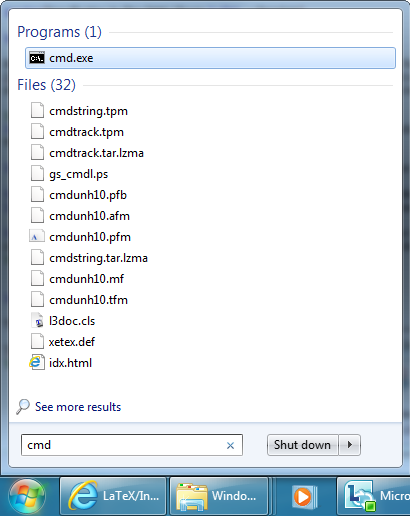
\includegraphics[scale=0.75]{TAMUthesis_CMD_windows.png}
% \caption[The command line compiler in Windows.]{The command line compiler in Windows. It is not suggested that you compile using this method. See compilation instructions in the README.}

% \label{fig:CMD_1}

% \end{figure}

% Figure (and table) titles should be consistent through the document. All
% captions should be placed either above or below the object it describes. This is
% done by placing the \textit{caption} in the correct place. While continued
% figures are allowed by the URS Thesis Manual with proper continuation headings, it is not suggested that any continued figures be included in a \LaTeX\ document.

% The figure below is taken from R. While there are packages available to import
% graphics from R, MATLAB, and similar software, it is probably best to export
% plots generated by these programs as a PNG file, and then import it via the
% \textit{includegraphics} command. Figures must also be referenced in the body
% text within 1 page of where the figure actually appears in the document.

% \begin{figure}[ht]
% 	\centering
% 	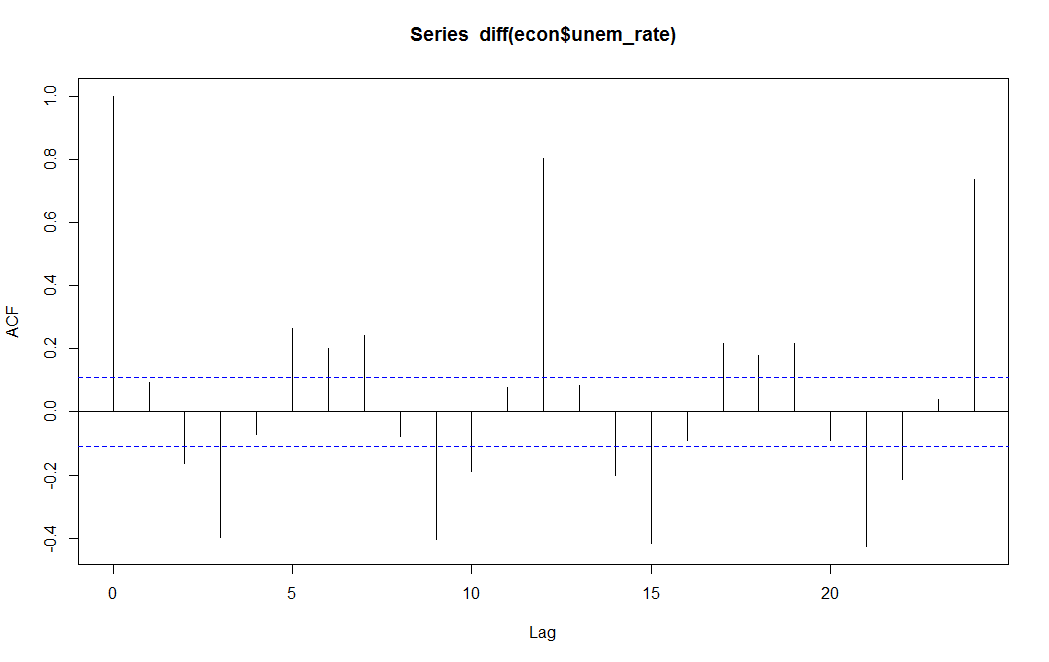
\includegraphics[scale=0.55]{UnemDiffACF.png}
% 	\caption{The autocorrelation function (ACF) of the differenced unemployment series. Seasonal adjustments may be needed.}
% \end{figure}

% \section{Table Placement, Size and Table Title}

% Here is a table, displaying band and auxiliary scores from the 2011 Arcadia Festival of Bands held in Arcadia, CA \cite{ARCADIA}.

% \begin{table}[h!]
% 	\centering

% 	\label{Band}
% 	\caption{Scores from the 2011 Arcadia Festival of Bands.}
%         \vspace{1em}
% 	\begin{tabular}{|l|l|l|}
% 		\hline
% 		School Name & Band Score & Auxiliary Score \\ \hline
% 		Rancho Bernardo & 96.15 & 89.15 \\ \hline
% 		Mt. Carmel & 95.30 & 83.55 \\ \hline
% 		Riverside King & 93.85 & 91.75 \\ \hline
% 		Diamond Bar & 93.20 & 88.60 \\ \hline
% 		El Dorado & 92.80 & 95.45 \\ \hline
% 		Chino & 92.65 & 91.45 \\ \hline
% 		Henry J. Kaiser & 92.60 & 87.55 \\ \hline
% 		Glendora & 92.60 & 89.15 \\ \hline
% 		Montebello & 90.50 & 82.70 \\ \hline
% 		Mira Mesa & 89.65 & 91.50 \\ \hline
% 	\end{tabular}
% \end{table}

% The table is sorted by band score. There is more text here to demonstrate how
% the template handles spacing between tables and body text. Also note how the
% table caption is in a smaller font size than the body text.

% \section{Equations}

% The following format is recommended to be used to display equations.

% %Make other examples.
% \begin{equation} \label{Equ.2.1}
% y=c_1\cos(t)+c_2\sin(t)
% \end{equation}
% \begin{equation} \label{Equ.2.2}
% e^{it}=\cos(t)+i\sin(t)
% \end{equation}

% Equation \ref{Equ.2.1} is the general solution to the differential equation $y''+y=0$. In the source code, the \textit{ref} command allows you to refer to an equation by a label you created. References must be made after the equation has been created; attempting to refer to an equation before it is defined results in a question mark placeholder. Some more sample equations are below. Notice the first set below is not numbered.
% %%
% \begin{align*}
% \log (x^n) &= \log (x \cdot x \cdot \ldots \cdot x) \\
% &= \log x + \log x + \ldots + \log x \\
% &= n \log x
% \end{align*}
% \begin{equation} \label{Equ.2.3}
% X^T X \mathbf{u} = X^T \mathbf{y}
% \end{equation}
% \begin{equation}\label{Equ.2.4}
% u(x, t) = \int_{-\infty}^{\infty} G(x, \tau) \exp\left(-\frac{(t-\tau)^2}{4kt}\right) \ d\tau
% \end{equation}
% \begin{gather}
% \mathcal{L}(f) = \int_{0}^{\infty} e^{-st} f(t) \ dt \\
% \begin{split} \label{Equ.2.5}
% \mathcal{F}(f) = \frac{1}{2\pi}\int_{-\infty}^{\infty} e^{i \omega x} f(x) \ dx
% \end{split}
% \end{gather}

% You can use labels to refer to equations you create. \ref{Equ.2.5} is the \textbf{Laplace transform} used extensively in differential equations. \ref{Equ.2.3} is the matrix representation of the \textbf{normal equations} used in least-squares regression.

% To have equations without labels appearing the right margin, simply add an asterisk to the name of the environment (equation, align, etc.) when making the declaration.


% \section{Theorems and Proofs: Examples}

% This section will show an example usage of the theorem and proof environments, typically used for mathematics students. To use these environments, you must have the package \textbf{amsthm} declared in the preamble of your document. For this template, this is already declared in the main file. You may choose to remove this declaration if your document will not make use of theorems and proofs.

% Theorems can be numbered, as the one below is, or you can force a different label to appear. For example, you can state the Bolzano-Weierstass theorem and have the names appear as the theorem label. See the examples below.

% Sometimes you may have a theorem with multiple parts or multiple conditions. You can use other list environments, such as enumerate, inside the theorem environment declared to list these conditions. The final example at the end of this block shows this with the Invertible Matrix Theorem, which has several equivalent statements.

% \renewcommand{\qedsymbol}{\rule{0.7em}{0.7em}}

% \newtheorem{thm}{Theorem}
% \begin{thm}
% 	Suppose $f$ is of class $\mathcal{C}^1$ and $g$ is of class $\mathcal{C}^2$, and that the compact set $D$ and its boundary satisfy the hypotheses of Green's Theorem.  Then
% 	\[ \iint \limits_D f\nabla^2 g \ dA = \oint_{\partial D} f(\nabla g) \cdot \mathbf{n} \ ds - \iint \limits_D \nabla f \cdot \nabla g \ dA . \]
% \end{thm}

% \begin{proof}
% 	Begin with the integral of $f\nabla g \cdot n$ taken over the boundary of D.  By the second vector form of Green's Theorem,
% 	\begin{align*}
% 	\oint_{\partial D} f\nabla g \cdot n \ ds &= \iint \limits_D \nabla \cdot (f\nabla g) \ dA \\
% 	&= \iint \limits_D f\nabla^2 g + \nabla f \cdot \nabla g \ dA.
% 	\end{align*}

% 	Rearranging yields the desired.
% \end{proof}

% \begin{thm}[Bolzano-Weierstrass]
% 	Every bounded real sequence has a convergent subsequence.
% \end{thm}

% \begin{thm}[Invertible Matrix Theorem\footnote{This is an incomplete list.}]
% 	For any square matrix $A$ with $n$ rows and columns, the following are equivalent.
% 	\begin{enumerate}
% 		\item $A$ is invertible.
% 		\item The equation $A\mathbf{x}=\mathbf{0}$ has only the trivial solution $\mathbf{x} = \mathbf{0}.$
% 		\item For any nonzero $\mathbf{b}, \ A\mathbf{x} = \mathbf{b}$ has exactly one solution.
% 		\item The columns of $A$ form a linearly independent set.
% 		\item Zero is not an eigenvalue of $A$.
% 		\item $A$ has full rank.
% 		\item The determinant of $A$ is not zero.
% 	\end{enumerate}
% \end{thm}

% There is currently no set format on how propositions and theorems should be laid out in the document. The idea is to remain consistent. It is best to not customize the appearance of theorems so that they can easily be distinguished from body text - just like figures, tables, and headings.

% \section{Another Table Example}
% For the sake of testing the appearance of the list of tables, a second table will be displayed here. This table displays a list of some major universities and their enrollments during fall 2015. This table is sorted in descending order of enrollment.
% %The savenotes environment, loaded from the footnote package
% %(which in turn is loaded from mdwtools)
% %allows you to use footnotes in tables, if needed.
% \begin{savenotes}
% \begin{table}[h!]
% 	\centering
% 	\label{my-label}
% 	\caption{Some major universities and their fall 2015 enrollments.}
%         \vspace{1em}
% 	\begin{tabular}{|l|l|l|}
% 		\hline
% 		School & City and State & Fall 2015 Enrollment  \\ \hline
% 		Texas A\&M University\footnote{Gig 'em!} & College Station, TX & 64,376  \\ \hline
% 		Ohio State University\footnote{This number describes enrollments at the Columbus campus; enrollments at regional campuses in Lima, Mansfield, Marion, Newark, and Wooster are not counted.} & Columbus, OH & 58,322 \\ \hline
% 		Iowa State University & Ames, IA & 36,001 \\ \hline
% 		University of California, San Diego & La Jolla, CA & 33,735   \\ \hline
% 		University of West Florida & Pensacola, FL & 12,798 \\ \hline
% 		Massachusetts Institute of Technology & Cambridge, MA & 11,319   \\ \hline
% 	\end{tabular}
% \end{table}
% \end{savenotes}

% Naturally, tables and footnotes do not go together. If you attempted to write a footnote inside a table, there will be nothing at the bottom of the page, yet the footnote marker will still appear. To remedy this, the \textit{footnote} package has been loaded from the \textit{mdwtools} package. Check your TeX distribution to see if \textit{mdwtools} is installed. See the source code for how this is implemented.
